\documentclass{article}

\usepackage[letterpaper,margin=1in,footskip=0.25in]{geometry}
\usepackage{fancyhdr}
\usepackage{tikz}
\usepackage{amsmath,mathtools}
\usepackage{csquotes}
\usepackage[hidelinks]{hyperref}
\usepackage{scrextend}

\usetikzlibrary{decorations.pathreplacing}

\MakeOuterQuote{"}

\deffootnotemark{\textsuperscript{[\thefootnotemark]}}
\deffootnote{2em}{1.6em}{\textsuperscript{\thefootnotemark}}

\newcommand{\dd}[2][]{\frac{\text{d}#1}{\text{d}#2}}
\newcommand{\dQ}{\text{d}Q}
\newcommand{\dt}{\text{d}t}
\newcommand{\e}[1][]{\text{e}^{#1}}

\pagestyle{fancy}
\fancyhf{}
\rfoot{Labalme \thepage}
\renewcommand{\headrulewidth}{0pt}

\begin{document}




\noindent Steven Labalme\\
\noindent Mr. Bilak\\
\noindent AP Physics C: Electricity and Magnetism, 6\\
\noindent 26 March 2019\\

\begin{center}
    \section*{RC Circuit Analysis}
\end{center}

\begin{figure}[h!]
    \centering
    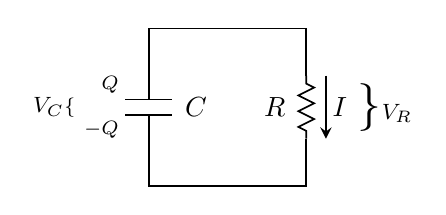
\begin{tikzpicture}[
        every path/.style={semithick},
        every node/.append style={inner sep=2pt}
    ]
        \draw (0,0) rectangle (2,2);

        \fill [white] (-0.3,0.9) rectangle node[black,xshift=6mm]{$C$} (0.3,1.1);
        \draw (-0.3,0.9) node[anchor=north east]{\scriptsize$-Q$} -- (0.3,0.9) (-0.3,1.1) node[anchor=south east]{\scriptsize$Q$} -- (0.3,1.1);

        \fill [white] (1.9,0.6) rectangle node[black,xshift=-4mm]{$R$} (2.1,1.4);
        \draw (2,0.6) -- (2,0.7) -- (1.9,0.75) -- (2.1,0.85) -- (1.9,0.95) -- (2.1,1.05) -- (1.9,1.15) -- (2.1,1.25) -- (2,1.3) -- (2,1.4);

        \draw [thick,-stealth] (2.25,1.4) -- node[right]{$I$} (2.25,0.6);

        \node at (-1.2,1) {\footnotesize$V_C$\scriptsize\{};
        \node at (3,1) {\LARGE\}\footnotesize$V_R$};
    \end{tikzpicture}
    \caption{A basic RC circuit.}
    \label{fig:RC}
\end{figure}

Consider the elementary RC circuit depicted in Figure \ref{fig:RC}. We seek to derive an expression for the magnitude of the charge $Q$ on either plate of the capacitor as a function of time $t$, as well as other values from Figure \ref{fig:RC} as needed.\par
To begin, analyze the circuit using Kirchhoff's Voltage Law. According to said law and WLOG\footnote{"Without the Loss Of Generality"}, analyze the circuit in a clockwise direction beginning in the bottom-left corner as indicated by Figure \ref{fig:RC}. This analysis will yield the following equation, where $V_C$ is the voltage gain across the capacitor and $V_R$ is the voltage drop across the resistor.

\begin{equation*}
    V_C-V_R=0
\end{equation*}

Let's express $V_C$ and $V_R$ in terms of other variables from Figure \ref{fig:RC}. Notably, $V_C$ can be related to $C$ and $Q$ through the definition of capacitance and $V_R$ can be related to $I$ and $R$ via Ohm's Law, as shown in Figure \ref{fig:tree}.

\begin{figure}[h!]
    \centering
    \begin{tikzpicture}[
        level 1/.style={sibling distance=7cm},
        edge from parent/.style={draw,latex-},
        every node/.style={anchor=south}
    ]
        \node {$\displaystyle\frac{Q}{C}-IR=0$} [grow'=up,child anchor=south]
            child {node {$
                \begin{aligned}
                    C &= \frac{Q}{V_C}\\
                    V_C &= \frac{Q}{C}
                \end{aligned}
            $}}
            child {node {$V_R = IR$}}
        ;
    \end{tikzpicture}
    \caption{Introducing more variables into the circuit analysis.}
    \label{fig:tree}
\end{figure}

We still need to find a way to introduce time. Fortunately, current is the time derivative of charge. While it might seem natural to substitute $\dd[Q]{t}$ for $I$, this will actually lead to an incorrect answer --- current is the rate at which charge $q$ passes through the circuit\footnote{Or, more formally, a cross section of a wire.}, not the rate of change of the magnitude of charge $Q$ on the plates of the capacitor. While it may now be tempting to substitute $\dd[q]{t}$ for $I$ and dismiss any relationship between $q$ and $Q$, the pair are intrinsically related.\par
In order to proceed, we must relate $q$ to $Q$. Let $\Delta q$ be a small quantity of charge that leaves the positive plate, passes through the circuit, and ends up on the negative plate. When $\Delta q$ leaves the positive plate, $Q$ decreases by $\Delta q$; in other words, the change in $Q$, $\Delta Q$, is equal to $-\Delta q$, or $\Delta Q = -\Delta q$. This is the relationship that we were looking for.\par
Both sides of the relationship $\Delta Q=-\Delta q$ can be differentiated with respect to time to relate said expression back to current $I$, as follows.
\begin{align*}
    \Delta Q &= -\Delta q\\
    \dd[Q]{t} &= -\dd[q]{t}\\
    \dd[Q]{t} &= -I\\
    I &= -\dd[Q]{t}
\end{align*}\par
Substitute the above definition of current into the resultant equation from Figure \ref{fig:tree}.
\begin{equation*}
    \frac{Q}{C}+\dd[Q]{t}R=0
\end{equation*}\par
Solve the above first-order differential equation for $Q$, as follows. Note that $Q_0$ is the charge on the plates at time $t=0$, while $Q$ is the charge on the plates at time $t$.
\begin{align*}
    \frac{Q}{RC}+\dd[Q]{t} &= 0\\
    \dd[Q]{t} &= -\frac{Q}{RC}\\
    \frac{\dQ}{Q} &= -\frac{1}{RC}\, \dt\\
    \int_{Q_0}^Q \frac{1}{Q}\, \dQ &= \int_0^t -\frac{1}{RC}\, \dt\\
    \left[ \ln(Q) \right]_{Q_0}^Q &= \left[ -\frac{t}{RC} \right]_0^t\\
    \ln(Q)-\ln(Q_0) &= -\frac{t}{RC}\\
    \ln\left( \frac{Q}{Q_0} \right) &= -\frac{t}{RC}\\
    \frac{Q}{Q_0} &= \e[-\frac{t}{RC}]\\
    \Aboxed{Q &= Q_0\e[-\frac{t}{RC}]}
\end{align*}

Note that the above equation holds true for $V$ and $V_0$, and $I$ and $I_0$, as well. These can be derived as follows\footnote{The substitutions are chosen and made based on the definition of capacitance and Ohm's Law.}.
\begin{align*}
    \frac{Q}{C} &= \frac{Q_0}{C}\e[-\frac{t}{RC}]&
        \frac{Q}{RC} &= \frac{Q_0}{RC}\e[-\frac{t}{RC}]\\
    \Aboxed{V &= V_0\e[-\frac{t}{RC}]}&
        \Aboxed{I &= I_0\e[-\frac{t}{RC}]}\\
\end{align*}




\end{document}